Automatic program synthesis has been a long term goal of the field of artificial intelligence since its inception \cite{mannaAutomaticProgramSynthesis1971}, promising to reduce the workload of software developers by automatically solving some of the tasks they face.
And since the field's inception it has been grappling with the challenging properties of the sparse optimization space \cite{alurSyntaxguidedSynthesis2013, davidProgramSynthesisChallenges2017} that is the set of all programs in a certain programming language, namely, 
\begin{enumerate}
    \item valid error-free programs constitute an exceedingly small part of the space of possible strings, so any program synthesis algorithm that incorporates random guessing (for instance, Reinforcement Learning with random initialization \cite{suttonReinforcementLearningSecond2018}) is exceedingly unlikely to guess a valid program;
    \item a small edit in a program can result in a large difference in it's behavior (and, conversely, the same algorithm can be expressed with very different programs), hence the programs we would like to find are not clustered in any compact part of the optimization space;
    \item some of the evaluation mechanisms of programs, especially in the \emph{Programmatically Interpretable Reinforcement Learning} paradigm involve stochasticity and can yield different results for the same program.
\end{enumerate}

In other words, the search space in program synthesis is \emph{sparse}, \emph{brittle} and sometimes \emph{noisy} \cite{arnoldNoisyOptimizationEvolution2002} - all known challenges in Optimization Theory.
Methods of program synthesis can be classified by how they address these challenges.

\newpage
\section{Genetic programming}
\label{sec:gp}

\begin{figure}[H]
    \centering
    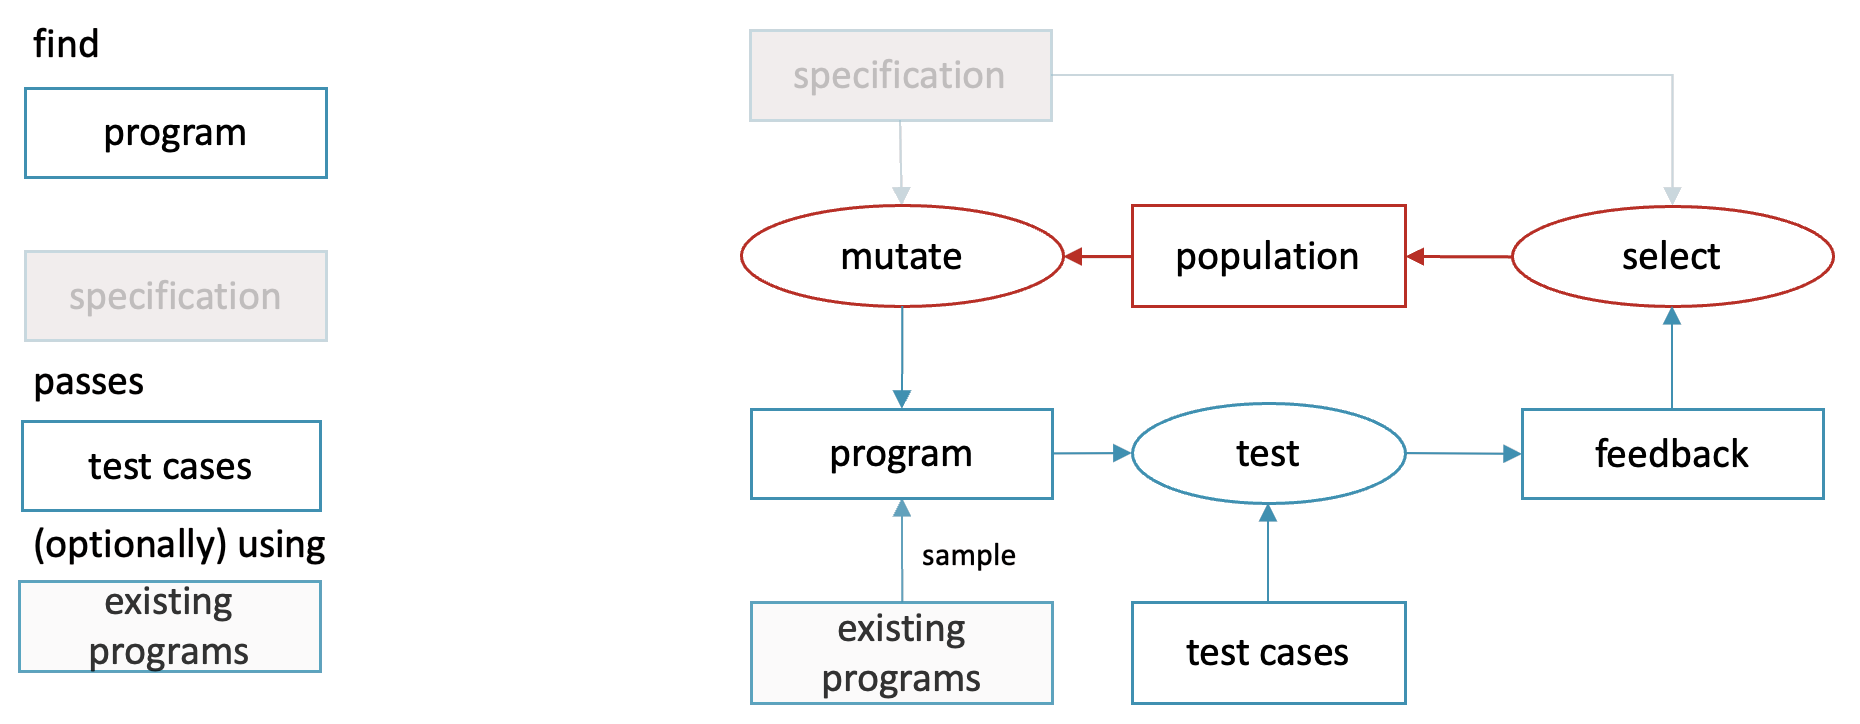
\includegraphics[width=\linewidth]{gp.png}
    \caption{Genetic Programming, schematic definition}
    \label{fig:gp}
\end{figure}

The family of optimization methods best applicable to this type of complex non-differentiable search space is \emph{genetic and evolutionary methods} - biologically inspired methods that operate on a population of candidate solutions (programs), randomly edit (\emph{mutation}) and combine (\emph{recombination}) to expand the population and the prune the population by \emph{natural selection}: removing the candidates that adhere to the specification the least.
Within program synthesis this family of methods is known as \emph{genetic programming} \cite{genprog1, genprog2, genprogast}
In an evolutionary setting, as soon as at least one (preferably several) valid program is found, initializing the population to include them drastically speeds up the search process, thus addressing the sparsity issue.
This approach is particularly powerful in a setting where some solutions are already known, but a program synthesis system can be used to search for solutions that fit the \emph{specification} even better, a setting known as \emph{genetic improvement of software} \cite{petke2018:genetic}.

Genetic programming has been successfully applied in various domains, including prediction and control \cite{dracopoulosGeneticProgrammingPrediction1997}, the synthesis of complex structures \cite{kozaHumancompetitiveApplicationsGenetic2003}, and the evolution of neural network modules \cite{degarisGENETICPROGRAMMING1990}. In the field of engineering, genetic programming has been applied to systems modeling, control, optimization, scheduling, design, and signal processing \cite{willisGeneticProgrammingIntroduction1997}. 

The biggest drawback of GP is that it requires generation and evaluation of a very high number of programs: higher than most other methods (see chapter \ref{ch:seidr}).
If evaluation of a generated program is computationally expensive, this translates directly into a very high computational cost of program synthesis.

\newpage
\section{Constrained programming languages}
\label{sec:constrainedpl}

Another way to address the complexity of the search space is to select a programming language such that the space of possible programs in that programming language exhibits less of the undesirable properties of optimization spaces.
For examples, a language where any combination of valid characters is a valid program \cite{brainfuck} eliminates a significant share of the complexity of the problem.
This family of approaches is explored in more detail in chapter \ref{ch:bfpp}, including  introduction of a novel constrained programming language for \emph{programmatically interpretable reinforcement learning}

\paragraph{Domain specific languages}

In some application domains it is common to express algorithms in domain specific programming languages \cite{fowlerDomainspecificLanguages2010, hudakDomainspecificLanguages1997, karsaiDesignGuidelinesDomain2014, kosarComparingGeneralpurposeDomainspecific2010, kosarDomainspecificLanguagesSystematic2016, mernikWhenHowDevelop2005} that tend to be more limited in terms of token vocabulary and grammatical complexity.
This provides the program synthesis community with a natural experiment in constraining the complexity of a language to simplify (automatic or manual) programming.
As a result, some of the most notable early positive results were in an industry standard database query language (SQL \cite{groffSQLCompleteReference2002}) \cite{liCanLlmAlready2024, yuSpiderLargescaleHumanlabeled2018} and an educational 2D robot control language (Karel \cite{pattisKarelRobotGentle1994}) \cite{metainduction}.

\paragraph{Logic programming}

One domain that's particularly amenable to solving synthesis tasks is \emph{logic programming}: a programming paradigm based on formal logic \cite{doetsLogicLogicProgramming1994, lloydFoundationsLogicProgramming2012}. 
In contrast to other programming paradigms \cite{floydParadigmsProgramming2007, gorodniaiaStudyProgrammingParadigms2016, krishnamurthi13ProgrammingParadigms2019, vanroyProgrammingParadigmsDummies2009} all functions in logic programming languages are boolean, which drastically limits the space of possible functions and makes many search-based approaches possible.

%Instead of (or in addition to) generating a program first and testing whether it adheres to specification, \emph{deductive} methods apply equivalence rules to translate the specification into an executable.
%This is hard to apply in \emph{programmatically interpretable reinforcement learning} where the specification is a black box, but can be a powerful approach in \emph{code translation} and \emph{programming by example} paradigms.


\newpage
\section{Unsupervised pre-training}
\label{sec:pretrain}

The paradigm of foundation models \cite{foundation-models} has recently been very prominent in machine learning and machine learning on source code is no exception.
In this paradigm, a model is first trained on a large dataset to solve a generic task such as next-token prediction and then used as a central component in solutions of various specific tasks.


\paragraph{Autoregressive models}

% Why this approach
Most modern foundation models are \emph{autoregressive}, i.e. trained to predict the a token in a program given all the preceding tokens.
This paradigm makes it easy to collect training data and parallelize computation.

% Architectures
\todo{Some words on architectures}

% Models
Autoregressive foundation models for source code, based on architectures such as GPT Codex \cite{radfordImprovingLanguageUnderstanding,chenEvaluatingLargeLanguage2021,codegen,gpt-neo} and BERT \cite{devlinBERTPretrainingDeep2019,codebert} have enabled significant process in tasks like programming by example \cite{halbertProgrammingExample1984} and even human-comparable performance in coding competitions \cite{liCompetitionLevelCodeGeneration2022}.

\paragraph{Autoencoder models}

While undoubtedly useful in many program synthesis tasks, popular foundation models may fall short in the areas of genetic programming \cite{genprogast} and genetic improvement of software \cite{petke2018:genetic}.
In these settings, new programs are found by exploring the space of programs similar to one or several reference programs.
The task of applying these perturbations to programs could benefit from a foundational model, however, it's unclear how to achieve this with the current autoregressive models.
Autoencoder Genetic Programming \cite{autoenc-gp,denoising-autoenc-gp,latentspaceopt} argues for using autoencoder \cite{autoencoders} models instead.
These models embed programs into a high-dimensional vector space, making it easy to mutate a program by add random noise to the embedding vector or combine several programs by averaging their embedding vectors.
Autoencoder-genetic programming is discussed in detail in chapter \ref{ch:tree2tree}.

\newpage
\section{Grammar guided synthesis}
\label{sec:grammar-guided}

Another way to constrain the hypothesis space is to use the grammar of the programming language in question directly in the program generation process.
Since in most implementations of compilers and interpreters, the first step of program execution is building an Abstract Syntax Tree representation of the code a software tool for AST parsing is available for most programming languages.

\begin{figure}[H]
    \centering
    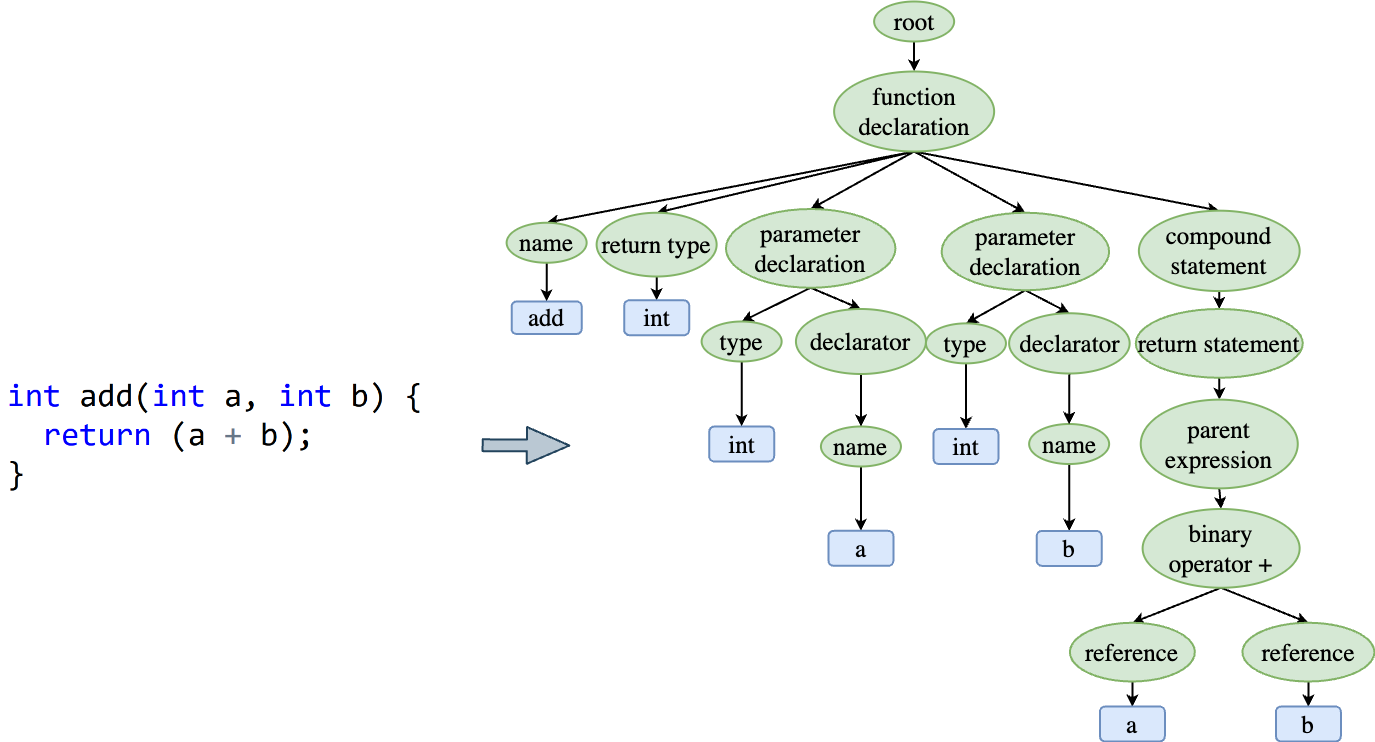
\includegraphics[width=\linewidth]{images/ast.png}
    \caption{Abstract syntax tree (AST) parser}
    \label{fig:ast-parser}
\end{figure}

When program synthesis systems  output ASTs, as opposed to raw text, a large class of errors (such as forgetting a semicolon) becomes impossible. 
Research literature on structural code encoding \cite{alon2019structural,zhang2015tree}, structural code decoding \cite{jiang2021ast,zhu2019grammarcnn} and grammar-guided genetic programming \cite{bunelLeveragingGrammarReinforcement2018, manriqueGrammarguidedGeneticProgramming2009, sobaniaChallengesProgramSynthesis2020a} suggests that models that operate directly on the tree structure of the program can achieve better performance than models that operate on a sequence of tokens.

A novel approach to grammar guided program synthesis is proposed in chapter \ref{ch:tree2tree}

\newpage
\section{Human in the loop}
\label{sec:human}

Alternatively, one can narrow the scope of the problem by retaining a human developer in the loop, but supporting them with CASE \cite{caseComputeraidedSoftwareEngineering1985} tools that solve some of the subtasks involved in developing a program.

\paragraph{Parametrization}

\todo{Probabilistic programming}

\todo{Differentiable programming}

\paragraph{Sketching}

\todo{Kevin Ellis goes here}

An \emph{autoregressive} language models lends themselves naturally to being used as a \emph{programming copilot}: a software tool integrated into the text editor as a core feature or an extension, that generates recommended code snippets based on the context (the code already present in the file).
At first glance \emph{copilots} may seem like a tool to accelerate typing, however, the developer can also imitate the "natural language to machine language" paradigm by describing the task at hand in a comment (or function name or docstring) and letting the copilot solve the task.

\todo{does "docstring" need to be explained?}

\begin{figure}[H]
    \centering
    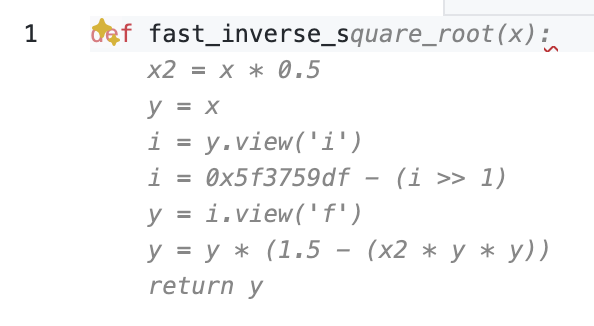
\includegraphics{images/fastinversesqrt.png}
    \caption{Github Copilot \cite{dakhelGithubCopilotAi2023, nguyenEmpiricalEvaluationGitHub2022, wermelingerUsingGithubCopilot2023} suggests an efficient algorithm for calculating inverse square root \cite{lomontFastInverseSquare2003} before the developer has finished typing the name of the method}
    \label{fig:fastinversesqrt}
\end{figure}

According to a large-scale survey \cite{liangLargeScaleSurveyUsability2024} \todo{what?}

\newpage
\section{Open problem}

The methods above have led to significant progress in \emph{code translation} and \emph{programming by example}, to the point where these paradigms have current industrial applications.
\emph{Programmatically Interpretable Reinforcement Learning}, however, largely remains an open problem.

\begin{highlight}
The goal of this thesis is to discover a methodology for Programmatically Interpretable Reinforcement Learning that can improve decision support systems in Healthcare and other safety-critical domains.
\end{highlight}


More concretely, we model the task as {\em Episodic Partially Observable Markov Decision Process}:

\begin{multline}
M = (\mathcal{S}_{nt}, \mathcal{S}_t, \mathcal{A}, \mathcal{O}, p_o(o | s, a), p_s(s_\text{next} | s_\text{prev}), p_r(r | s, a), p_\text{init}(s))
\end{multline}

Here, $\mathcal{S}_{nt}$ is the set of {\em non-terminal (environment) states} and $\mathcal{S}_{t}$ is the set of {\em terminal states}. 
$\mathcal{A}$ is the set of {\em actions} that the learning agent can perform, and $\mathcal{O}$ is the set of {\em observations} about the current state that the agent can make. 

A \emph{reinforcement learning episode} starts in a state $s \in \mathcal{S}_{nt}$ sampled from $p_\text{init}$, the {\em initial distribution} over environment states.
An agent action $a \in \mathcal{A}$ at the state $s$ causes the environment state to change probabilistically, and the destination state follows the distribution $p_s(\cdot | s, a)$. 
At state $s$, the probability of making observation $o$ is $p_o(o | s)$ and the probability of obtaining \emph{reward} $r$ is $p_r(r|s,a)$. 
The process continues until a $p_s$ yields a terminal state $s \in \mathcal{S}_t$.
This distinction is what sets \emph{episodic} POMDP popularized by OpenAI gym \cite{openai-gym} apart from the more traditional approach \cite{kramerjdavidrPartiallyObservableMarkov1964, spaanPartiallyObservableMarkov2012} where the process is infinite.

A \emph{program} is a sequence of tokens

\begin{equation}
    \code=(\code^{(1)},\code^{(2)},\dots)
\end{equation}

that defines behavior of an agent.
Depending on the programming language and implementation choices the tokens can be characters or higher-level tokens, i.e. keywords.
We denote the language's \emph{alphabet}, i.e. the set of all possible tokens as $\mathcal{L}$.

An \emph{interpreter} is a tuple $\langle \alpha,\mu \rangle$ where $\mu(c_k,m_k,o_k)$ is the \emph{memorization function} that defines how the agent's memory updates upon making an observation and $\alpha(c, m_k)$ is the \emph{action function} defines which action the agent at a certain memory state takes in the POMDP.
Memory is intialized at state $m_\text{init}$

The agent's goal is maximizing total reward collected in the environment, calculated as follows:

\begin{algorithm}[H]
\begin{algorithmic}[1]
\caption{Evaluating total reward for a program}
\Function{$\mathit{Eval}$}{$c$}
\State $R_\text{tot} \gets 0$
\State $m \gets m_\text{init}$
\State $s \sim p_\text{init}(s)$
\While{$s \in \mathcal{S}_{nt}$}
\State $o \sim p_o(o | s)$
\Comment{Observe}
\State $m \gets \mu(c,m,o)$
\State $a \gets \alpha(c, m)$ 
\Comment{Act}
\State $r \sim p_r(s,a)$
\State $R_\text{tot} \gets R_\text{tot} + r$
\Comment{Get rewarded}
\State $s_\text{next} \sim p_s(s_\text{next} | s, a)$
\Comment{Next state}
\State $s\gets s_\text{next}$
\EndWhile
\State \Return $R_\text{tot}$
\EndFunction
\end{algorithmic}
\end{algorithm}

Since the algorithm for computing this function involves repeatedly sampling values from distributions, function $\mathit{Eval}(c)$ is a mapping from the set of programs to the set of real-valued random variables.

\emph{Programmatically Interpretable Reinforcement Learning} \cite{pirl} is the task of maximizing expected total reward with respect to $c$, i.e. finding a program $c$ that is best for a given POMDP environment:

\begin{equation}
    \expectation(\mathit{Eval}(c)) \longrightarrow \max_{c}
    \label{eq:pirlgoal}
\end{equation}

The following chapters assume the framework above.
Chapter \ref{ch:bfpp} introduces a domain specific language for program synthesis. 
Chapter \ref{ch:neurogen} introduces a combination of neural program synthesis and genetic programming to synthesize better programs in this and other languages.
Chapter \ref{ch:tree2tree} attempts to use grammar-guided autoencoder program synthesis to extend this method to industry-standard programming languages.
Chapter \ref{ch:seidr} takles the same problem with autoregressive Large Language Models instead and achieves state of the art results in Programmatically Interpretable Reinforcement Learning.
Chapter \todo{} discusses the importance of simulator-driven PIRL for Smart Healthcare.
Chapters \todo{} introduces a Reinforcement Learning environments for  emergency care.
Chapter \todo{} applies the method from chapter \ref{ch:seidr} to the emergency care environment and demonstrates the potential of Programmatically Interpretable Reinforcement Learning in Healthcare.
However, this environment is based on models developed by experts and can be subject to expert biases.
To address this limitation, chapter \todo{} introduces a fully data-driven benchmark for future work in the area.